
\section{Results}

Here, We have the result of quantitative measures to assess the level of agreement between the data and the simulation, using amplitude and slope parameters. A python program is developed to produce plots of all the available pairs of data and synthetics attenuation relationship comparision, and also to compare all four velocity models together.Fig.~\ref{fig:pgv} shows results of PGV in total (average of 3 directions) for all 4 models as an example. As it can be seen, the four models have close regression lines in most of the cases.

\begin{figure*}
    \centering
    \includegraphics
    	[width=\textwidth]
    	{figures/pdf/figure-02}
    \caption{PGV for all the 30 events and all four models are presented.}
    \label{fig:pgv}
\end{figure*}

For the first set of trials the t prameter was calculated. Then, considering the variations in the t value ranges, an initial score is proposed corresponding to each t. Current selected ranges are: 10 if $0 \leq t\leq 0.1$, 9 if $0.1 < t\leq 1$, 8 if  $1 < t\leq 10$, 7 if  $10 < t\leq 20$, 6 if  $20 < t\leq 100$ and 5 if  $100 < t\leq 500$. Later it will be an acceptable function of t for calculating score instead of just assigning the score for different t ranges. This will make the GOF more accurate and applicable.

In order to better see the changes in amplitude score, rate score, and total score using a python program plots for the trend of changes in all 30 events are produced. Here some of them are discussed with the aim of comparing four different velocity models. Fig.~\ref{fig:amp} shows trend of amplitude score for PGD, PGV and PGA for all 4 models. In all of them the same trend is visible. PGD has better scores, then PGV, then PGA. Among all cvms426-223 has better overall result.

\begin{figure*}
    \centering
    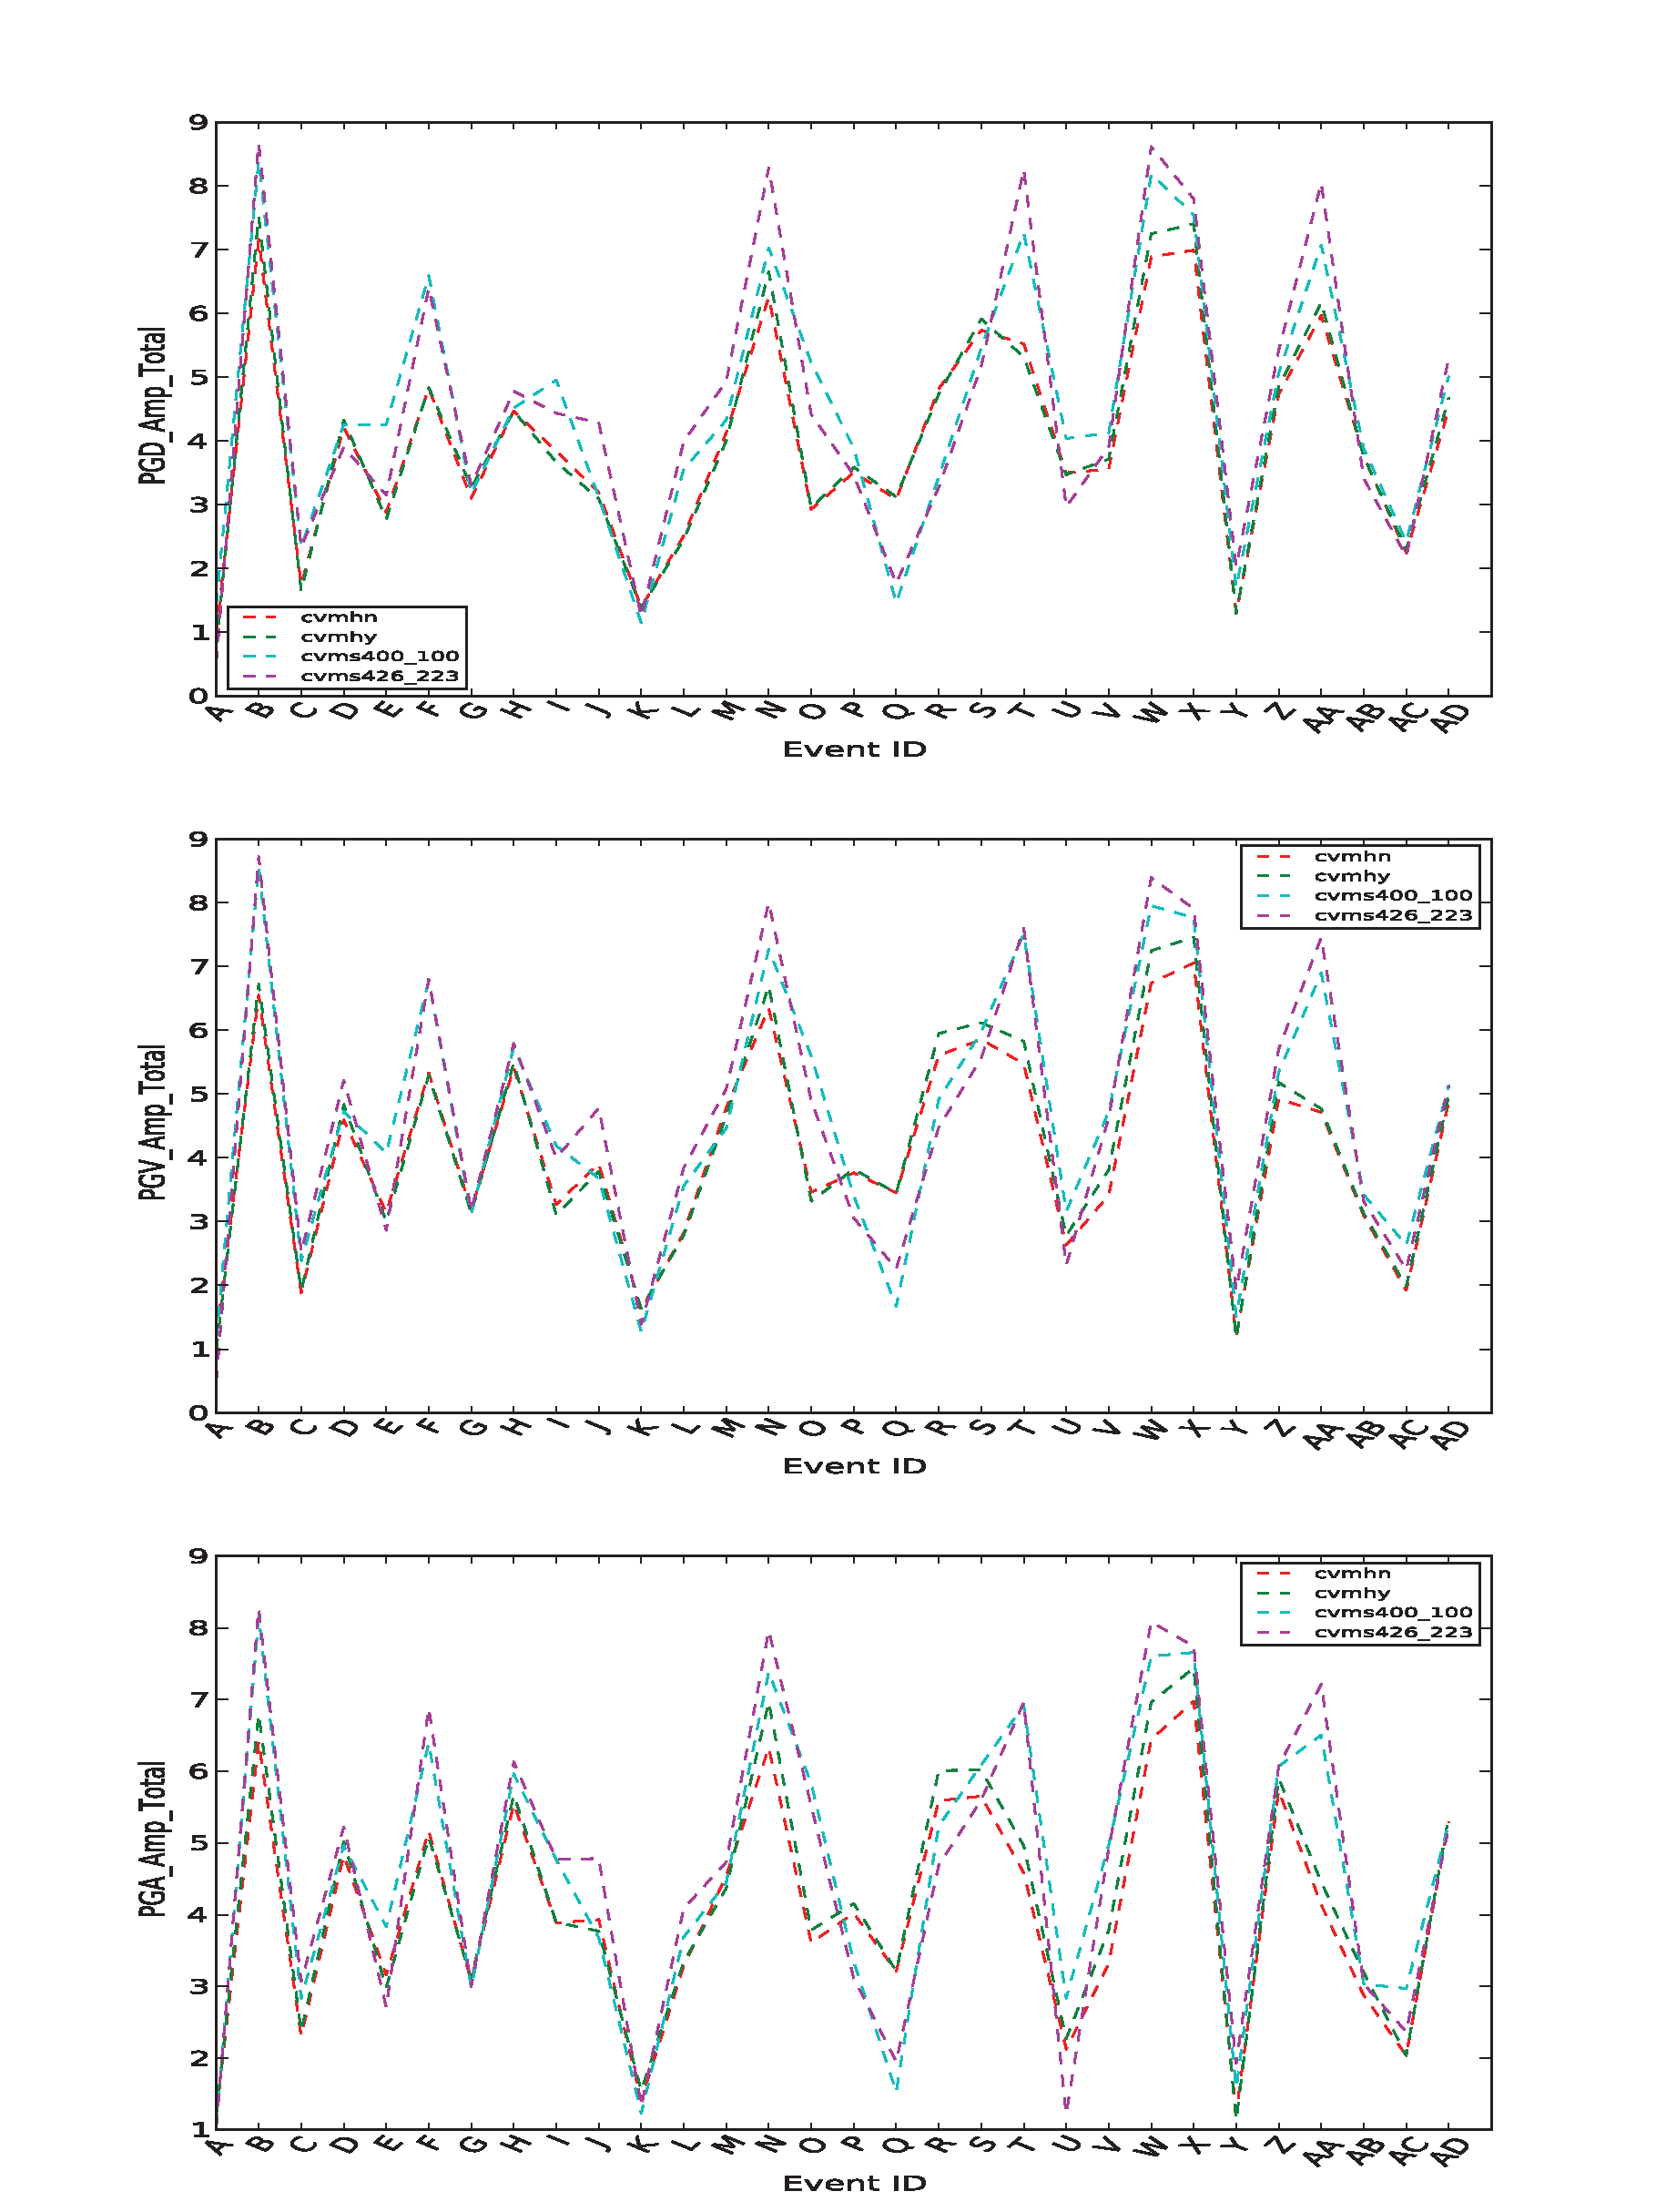
\includegraphics
    	[width=\textwidth]
    	{figures/pdf/figure-03}
    \caption{PGD, PGV and PGA amplitude score for all the 30 events and all four models are presented.}
    \label{fig:amp}
\end{figure*}

 Fig.~\ref{fig:rate} shows trend of rate score for PGD, PGV and PGA for all 4 models. PGD still has better scores then PGV, then PGA. Bur we can see different trends here.

\begin{figure*}
    \centering
    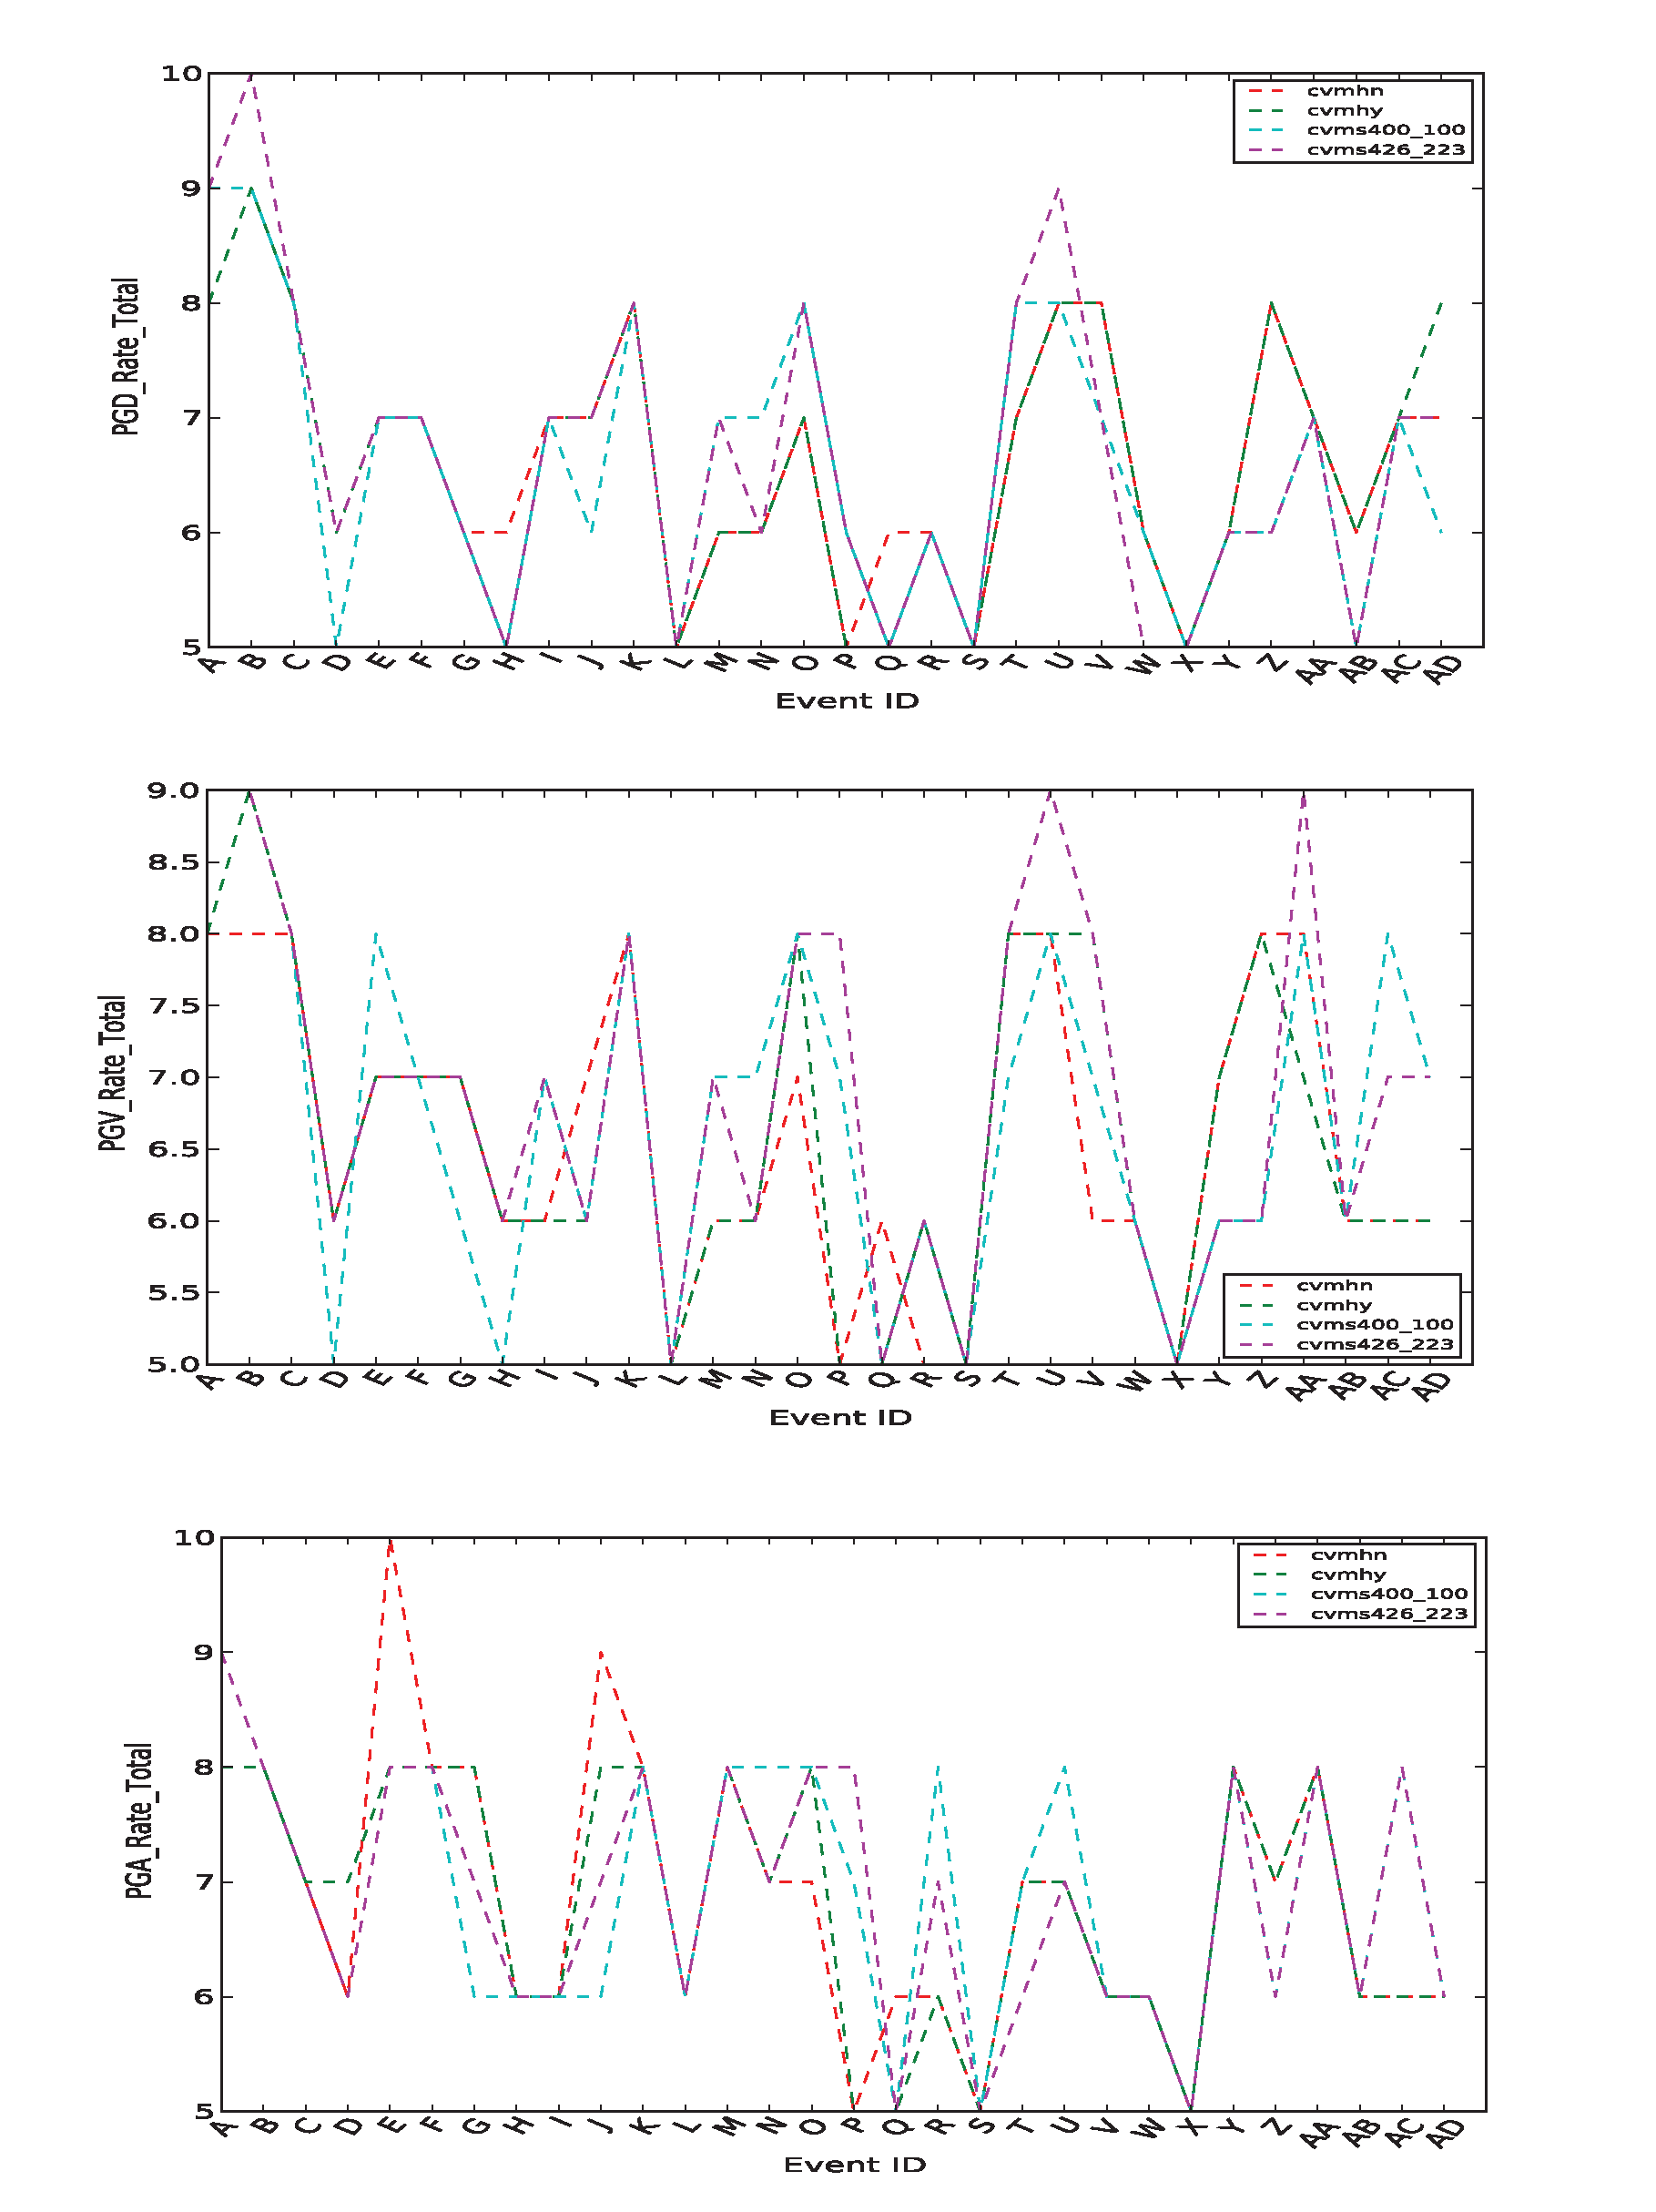
\includegraphics
    	[width=\textwidth]
    	{figures/pdf/figure-04}
    \caption{PGD, PGV and PGA rate score for all the 30 events and all four models are presented.}
    \label{fig:rate}
\end{figure*}

 Fig.~\ref{fig:score} shows trend of total average score for PGD, PGV and PGA for all 4 models. Again, the trend is similar, the score is better in PGD, then PGV, then PGA, and CVMS426-223 shows a better overall results.


\begin{figure*}
    \centering
    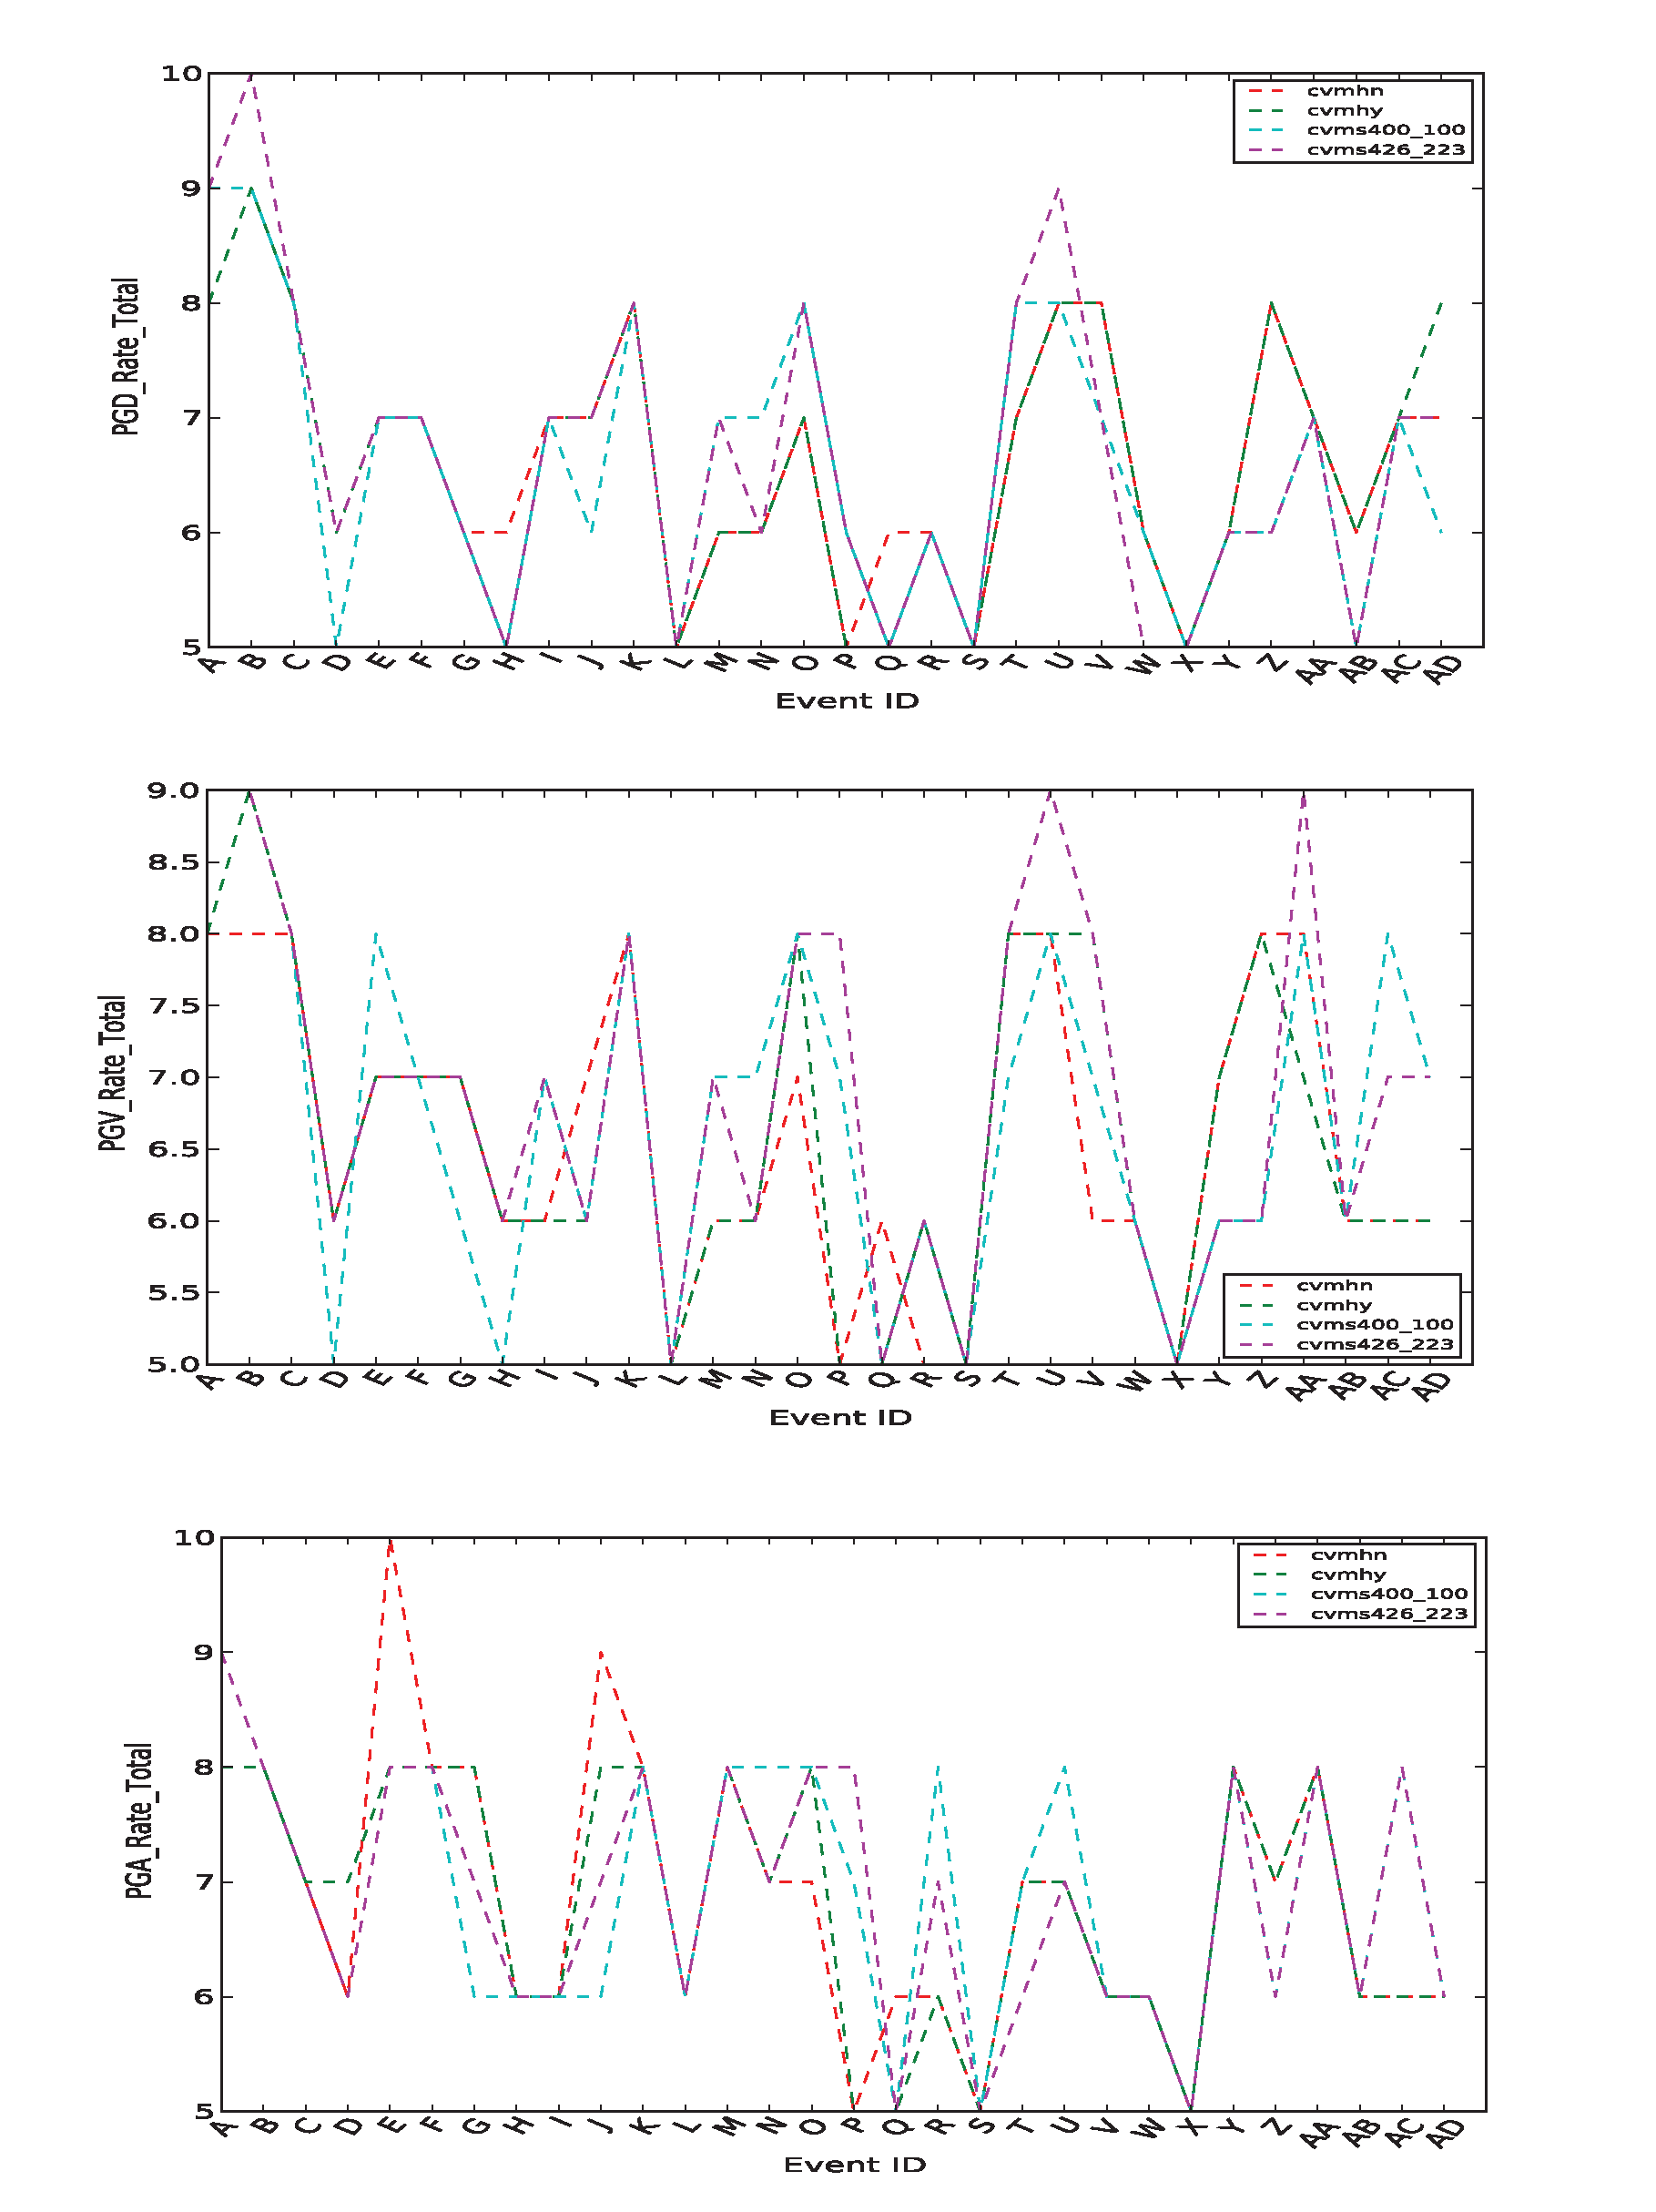
\includegraphics
    	[width=\textwidth]
    	{figures/pdf/figure-05}
    \caption{PGD, PGV and PGA total average score for all the 30 events and all four models are presented.}
    \label{fig:score}
\end{figure*}


A comparision between the latest results from scores of validation with modified anderson method and the method proposed here shows a good compatibility between final results of both methods. (See figure \ref{fig:comparision})

\begin{figure*}
    \centering
    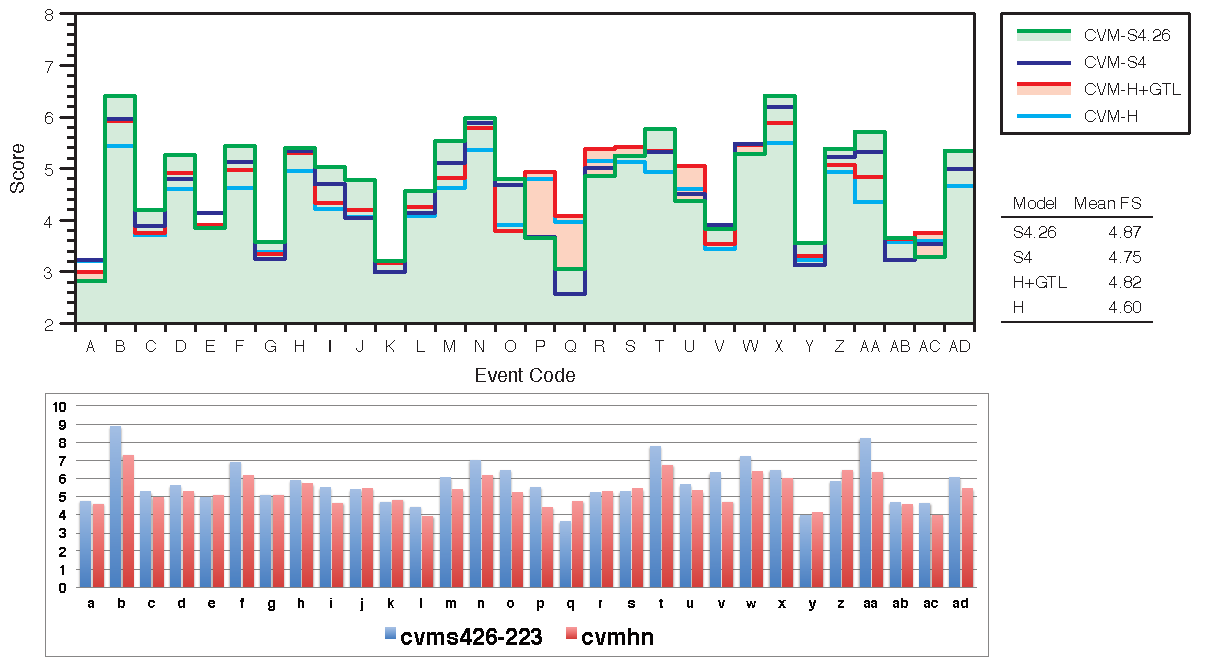
\includegraphics
    	[width=\textwidth]
    	{figures/pdf/figure-06}
    \caption{Results from modified Anderson score at top and the proposed score here for PGV at bottom}
    \label{fig:comparision}
\end{figure*}
